\documentclass[12 pt]{article}

\usepackage{enumerate} 
\usepackage[utf8x]{inputenc}
\usepackage[spanish,mexico]{babel}
\usepackage{amsmath}
\usepackage{amssymb}
\usepackage{enumitem}
\usepackage{amsthm}

\usepackage{listings}
\usepackage{minted}

\usepackage{graphicx}
\usepackage{python}
\usepackage{etoolbox}
\patchcmd{\endpython}{python }{python3 }{}{}


\title{Simulación - Segunda tarea}
\author{Sergio Arnaud Gómez \quad \quad \ 159189}
\date{10 de septiembre del 2018}

\newtheorem{teo}{Teorema}
\newtheorem{lema}[teo]{Lema}
\renewcommand\qedsymbol{$\null\hfill\blacksquare$}

\begin{document}
\maketitle
\begin{enumerate}
    

    \item Probar por inducción que para un GLC:
    
    \[ Z_i \equiv \left[a^iZ_0 + c\frac{a^i - 1}{a - 1}\right] mod \ m \] 
    
    \underline{Demostración:} (Por inducción sobre i)
    
    (Base de inducción) si $i=0$ tenemos que:
    \begin{align*}
        a^iZ_0 + c\frac{a ^i - 1}{a - 1} &=
        a^0Z_0 + c\frac{a^0 - 1}{a - 1}\\ &=
        Z_0 + c\frac{1 - 1}{a - 1} \\ &=
        Z_0 \\ &\equiv Z_0 \ mod  \ m
    \end{align*}
    
    De forma que para i = 0 tendremos 
    
    (Hipótesis de inducción) Ahora supongamos que el resultado válido para $i=n$ y probemos la afirmación para $n+1$. 
    
    Por un lado, por la definición de los generadores lineales congruenciales tendemos que :
    \begin{align*}
        Z_{n+1} \equiv (aZ_n + c) \ mod \ m \tag{1} \label{eq:1}
    \end{align*}
    
    Por otro lado, por la hipótesis de inducción tenemos que:
    \begin{align*}
        Z_n \equiv \left[a^nZ_0 + c\frac{a^n - 1}{a - 1}\right] mod \ m 
    \end{align*}
    
    Trabajando con esta última expresión obtenemos:
    \begin{align*}
        & & Z_n &\equiv \left[a^nZ_0 + c\frac{a^n - 1}{a - 1}\right] mod \ m \\
        & \implies & aZ_n &\equiv a\left[a^nZ_0 + c\frac{a^n - 1}{a - 1}\right] mod \ m \\
        & \implies & aZ_n + c &\equiv a\left[a^nZ_0 + c\frac{a^n - 1}{a - 1}\right] + c mod \ m \\
        & \iff & aZ_n + c &\equiv \left[a^{n+1}Z_0 + c\frac{a^{n+1} - a}{a - 1} + c\right] mod \ m \\
        & \iff & aZ_n + c &\equiv \left[a^{n+1}Z_0 + c\frac{a^{n+1} - 1}{a - 1} \right] mod \ m  \tag{2} \label{eq:2} \\ 
    \end{align*}
    
    Dado que la relación de congruencia es, en particular, una relación de equivalencia se tiene la transitividad y por las ecuaciones \eqref{eq:1} y \eqref{eq:2} concluimos la demostración al obtener:
    \begin{align*}
        Z_{n+1} \equiv \left[a^{n+1}Z_0 + c\frac{a^{n+1} - 1}{a - 1} \right] mod \ m 
    \end{align*} 
    \qedsymbol
    
    \newpage
    
    \item¿Qué se puede decir de el periodo de $Z_i \equiv aZ_{i-1}\ mod \ m$  con $a = 630,360,016$ y $m = 2^{31} -1$
    
    Dado que es un GLC multiplicativo no cumple el teorema del periodo completo (c = 0 por lo que no es primo relativo con m) de forma que el periodo máximo que podría alcanzar es m-1
    
    \newpage
    
    \item Sin calcular ninguna $Z_i$, determinar cuál de los siguientes GLC’s mixtos tienen periodo completo.
    
    \begin{enumerate}[label=(\alph*)]
        \item $Z_i \equiv [13Z_i + 13] \ mod \ 16$
        \item $Z_i \equiv [12Z_i + 13] \ mod \ 16$
        \item $Z_i \equiv [13Z_i + 12] \ mod \ 16$
        \item $Z_i \equiv [Z_i + 12] \ mod \ 16$
        \item $Z_i \equiv [aZ_i + c] \ mod \ m$ con $a = 2814749767109$, $c = 59482661568307$ y $m =2^{48}$
        
    \end{enumerate}
    
    \underline{Solución:}
    
    Para resolver dicho problema se realizó una función en python que permite saber si un GLC tiene periodo completo o no, lo hace tras verificar que cumpla las 3 hipótesis del teorema del periodo completo, es decir, verifica:
    
    \begin{enumerate}
        \item Que c y m son primos relativos
        \item Que si q es un número primo que divide a m, entonces q también divide a − 1 (a ≡ 1)
              mod q, para cada factor primo de m.)
        \item Finalmente, que si 4 divide a m, entonces 4 divide a − 1. (a ≡ 1 m´od 4, si 4 divide a m).
    \end{enumerate}    

    El programa está escrito en python 3 y el código fuente se muestra a continuación:
    
    \inputminted[fontsize=\small]{python}{complete_period.py}
    
    \newpage
    Tras ejecutar el programa en los ejercicios proporcionados se obtuvo que los generadores dadas por las expresiones a), d) y e) tienen periodo completo mientras que los dados por b) y c) no, a continuación se muestran los resultados

    \begin{figure}[h]
        \centering
        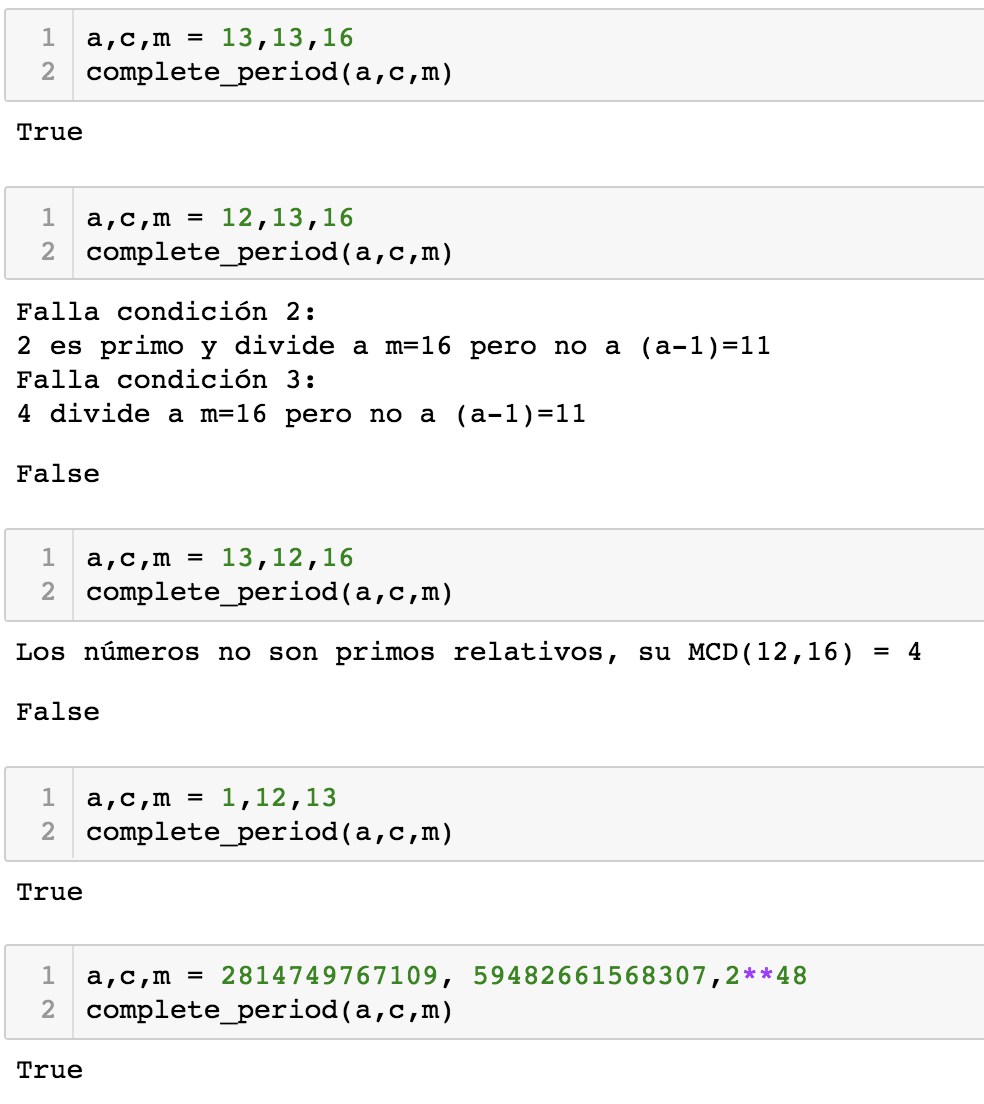
\includegraphics[width=11.5cm]{output_3.png}
    \end{figure}
    
    \newpage
    
    
    \item Mostrar que el promedio de las $U_i’s$ tomadas de un ciclo completo de un GLC de periodo completo es $\frac{1}{2} - \frac{1}{m} $
    
    \underline{Demostración:}
    
    Afirmación: Dado un generador de ciclo completo, si $Z_i \equiv$ $\left[a^iZ_0 + c\frac{a^i - 1}{a - 1}\right] mod \ m$ entonces $\{ Z_i \ | \ 0 \leq i < m, \} = \{0,1,...,m-1\}$. Para probar dicha afirmación basta notar que por un lado $\{ Z_i \ | \ 0 \leq i < m, \} \subset \{0,1,...,m-1\}$ por la definición de los $Z_i's$. Por otro lado $\{0,1,...,m-1\} \subset \{ Z_i \ | \ 0 \leq i < m, \} $ pues en caso contrario el generador no sería completo. 
    
    Con dicha afirmación, tenemos: 
    \begin{align*}
        \frac{1}{m}\sum_{i=1}^{m} U_i &= \frac{1}{m}\sum_{i=1}^{m} \frac{Z_i}{m} \\
        &= \frac{1}{m^2}\sum_{i=1}^{m}  Z_i  \\
        &= \frac{1}{m^2}\sum_{i\in\mathbb{N}, i<m} i \\
        &= \frac{1}{m^2} \frac{(m-1)(m)}{2} \\
        &= \frac{(m-1)}{2m} \\
        &= \frac{m}{2} - \frac{1}{2m}
    \end{align*}
    \qedsymbol
    
    \newpage
    
    \item Generar 10,000 números con U (0, 1) de Excel. Hacer un breve estudio para probar la calidad de los generadores; aplicar las pruebas de uniformidad e independencia a cada conjunto de datos. Resumir resultados en NO MAS de 2 cuartillas, incluyendo gráficas. De acuerdo a tus resultados, ¿cómo calificarías al generador de Excel?
    
    \newpage
    \item Probar que la parte fraccional de la suma de uniformes en $[0,1]$: $U_1 + U_2 + ... + U_k$ es también uniforme en el intervalo $[0,1]$.
    
    \newpage
    \item Un generador de Fibonacci obtiene $X_{n+1}$ a partir de $X_n$ y $X_{n−1}$ de la siguiente forma:
    
    \begin{align*}
        X_{i+1} = (X_i + X_{i-1}) \ mod \ m
    \end{align*}
    
    Con $X_0$ y $X_1$ dados. Para $m=5$ solo dos ciclos son posibles, encontrarlos y al periodo.
    
    \underline{Solucion:}
    
    Para la solución a dicho problema se implementaron las siguientes funciones en python3
    
    \inputminted[fontsize=\scriptsize]{python}{fibonacci_generator.py}
    
    La función "fibo" recibe como parámetros $X_0$ y $X_1$, las raíces y m, el módulo. Y genera el los números producidos por la iteración hasta caer en un ciclo, como ejemplos:
    
    \begin{figure}[h]
        \centering
        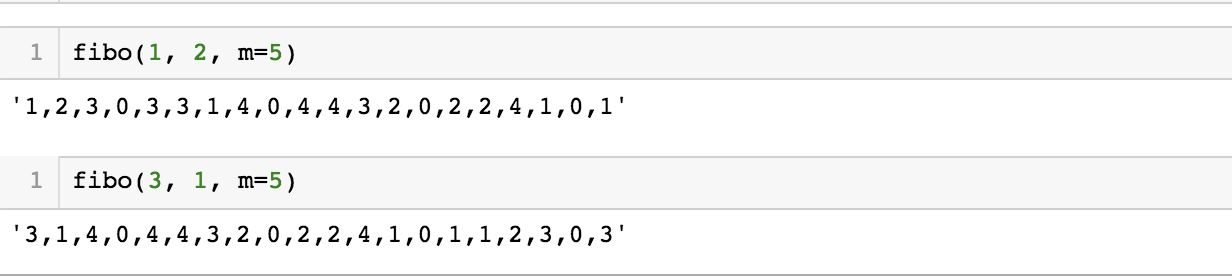
\includegraphics[width=11cm]{fibonacci.png}
    \end{figure}
    
    Haciendo uso de dicha función, la siguiente función obtiene todos los posibles ciclos de el generador de fibonacci para un n dado, para $n=5$ tenemos los siguientes resultados:
    
    \begin{figure}[h]
        \centering
        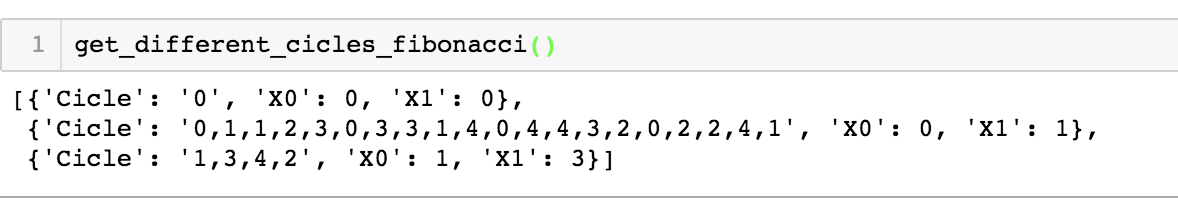
\includegraphics[width=11cm]{cicles.png}
    \end{figure}
    
    Notamos que, además del ciclo trivial, hay 2 ciclos distintos.
    
    \newpage
    
    \item Genera 10,000 números con una semilla de $Z_0 = 1$ usando el generador $Z_n = 75Z_{n-1} \ mod  \ (2^{31} −1)$ Clasifica los números en 10 celdas de igual tamaño y prueben por  uniformidad usando la prueba $\xi^2$ con un nivel de confianza del 90\%. Aplicar también la prueba de rachas.
    
    \underline{Solución}

    <<cache=TRUE>>=

    GLC = function(z0,a,c,m,k){
        
        df = data.frame(Ui = z0/m)
        z = (z0*a + c)%%m
        for (i in 2:k){
            df = rbind(df, data.frame(Ui = z/m))
            z = (z*a + c)%%m
        }
        return (df)
    }

    df = GLC(1,7^5,0,2^31-1,10000)
    head(df)

    h = hist(df$Ui, breaks = 10, right = FALSE, plot = FALSE)
    breaks_cdf <- punif(h$breaks)
    null.probs <- breaks_cdf[-1] - breaks_cdf[-length(breaks_cdf)]
    a <- chisq.test(h$counts, p = null.probs, rescale.p = T,
    simulate.p.value = T)
    a
    @
    
\newpage
    
    
    
\end{enumerate}



\end{document}
